\documentclass[11pt]{article}
\usepackage[margin=0.75in]{geometry}
\usepackage{amsmath}
\usepackage{amssymb}
\usepackage{setspace}
\usepackage{graphicx}

\usepackage{color}
\definecolor{deepblue}{rgb}{0,0,0.5}
\definecolor{deepred}{rgb}{0.6,0,0}
\definecolor{deepgreen}{rgb}{0,0.5,0}
\usepackage{listings}

\DeclareFixedFont{\ttb}{T1}{txtt}{bx}{n}{12} % for bold
\DeclareFixedFont{\ttm}{T1}{txtt}{m}{n}{12}  % for normal

% Python style for highlighting
\newcommand\pythonstyle{\lstset{
    language=Python,
    basicstyle=\ttm,
    otherkeywords={self},             % Add keywords here
    keywordstyle=\ttb\color{deepblue},
    emphstyle=\ttb\color{deepred},    % Custom highlighting style
    stringstyle=\color{deepgreen},
    frame=tb,                         % Any extra options here
    showstringspaces=false            % 
}}


% Python environment
\lstnewenvironment{python}[1][]
{
    \pythonstyle
    \lstset{#1}
}
{}

    

\begin{document}

\title{ECE 4750 Lab 1: Iterative Integer Multiplier}
\author{Akshay Dongaonkar (akd54) \& Avinash Navada (abn44) \& Vivek Gaddam (vrg22)}
\maketitle

\section{Introduction}

In many programming algorithms, multiplication is a key step in driving the algorithm towards completion. 
Many digital signal processing algorithms spend most of their time multiplying values. 
Given our media heavy, highly connected Internet of Things (IoT), more signals will need to be processed.
Therefore, we have synthesized an iterative multiplier that supports the mul instruction as defined in the PARCv1 Instruction Set Architecture (ISA).
Eventually, this multiplier will be a module in a fully synthesizable multicore processor.

We implemented two multiply designs: the first is a fixed latency, 34 cycle iterative multiplier while the second is a variable latency
iterative multiplier with bounds of 3 to 34 cycles.
While we do not expect much additional overhead on clock frequency in our variable multiplier,
we expect a significant increase in area and energy.
Given the technology constraints we face today, (focus on energy, large die sizes, etc),
we expect our variable multiplier to be superior in most implementations. 


\section{Project Management}

Given our group's various skill levels, we assigned Avinash to be verification lead, Vivek to be the architect, and Akshay to be the design lead.
Our initial project roadmap was fairly aggressive and required us to be finished by Wednesday, September $10^{th}$.
The intial Gantt Chart is shown in Figure~\ref{fig:gantt}.

The breakdown of work in our group followed as such:
Vivek implemented most of the baseline design and some of the alternate design in Verilog. 
Avinash implemented some of the alternate design and created our testing suite for lab 1.
Akshay came up with the designs for the multiple alternate designs and wrote most of the writeup.
Akshay also helped debug the Verilog code; Vivek figured out more than half the errors though.

As far as implementing the lab, most of it was tested via an end to end fashion.
 


\section{Baseline Design}

The baseline design works on the following interface: 
given a 64 bit message containing our operands, a clock signal,
and required signals to conform to the val/rdy microprotocol,
output the lower 32 bits of the multiplication to your consumer.
This interface is shown in Figure~\ref{fig:model}.
Our algorithm for computing the multiplication is as follows.
If the least significant bit (lsb) of the second operand (call it $b$) is 1, add it to an accumulator.
Then, shift your first operand (call it $a$) left by one bit and the second operand to the right logically by one bit.
This is the first algorithm we are taught when we learn to multiply.
The pseudocode for this is shown in Figure~\ref{fig:code}. 

Our implementation follows the structure of this pseudo-code very closely.
We have three registers, one each for $a$, $b$, and $result$ (our accumulator).
We have 2 shifters, one logical left shifter and one logical right shifter. 
We have an equivalent multiplexor for the clause that adds to our accumulator if the lsb of $b$ is $1$.

However, the control logic and the data flow are not implemented as a monolithic design.
Instead, we implement a \textit{control-datapath split.}
The control module sends control signals to the datapath module, altering the flow of data into the registers.
This occurs when we are accepting new values into our operand registers,
writing/not-writing partial sums to $result$, and outputing a computed value.
The datapath module sends the lsb of $b$ to the control module so it can compute the appropriate dataflow.
It is shown in Figure~\ref{fig:datapath}.
The lsb is directly used to determine whether to partially sum into $results$, a direct mapping to the pseudocode.

As seen from the pseudocode, there is no escape from the \verb+for+ loop.
Therefore, this implementation \textbf{must} take at least 32 cycles.
In fact, our implementation takes 34 cycles, as we have one cycle to accept data and one cycle to state we are done.
The state machine capturing this logic is shown in Figure~\ref{fig:state}. 
This implementation, therefore, does exploit patterns in the underlying data.
In the most extreme case where $b$ is zero, the hardware checks every bit of $b$ and decides 32 times not to add to $result$.
We should reduce that down to one decision not to write to $result$.

Another slight disadvantage to our baseline design was the failure to identify and exploit repeated structures into modularity.
Notice that each register has a multiplexor in front of it directing output.
We should have wrapped that structure into a module and reused it three times. 
This would have allowed us to test incrementally and unit-by-unit.
Instead, we were forced to rely on end-to-end testing and test all functionality at once.
As a consequence, we ran into a Verilog bug that took several hours to fix even with help.  
 

\section{Alternative Design}

The primary downside to our baseline implementation is the large latency in computing the product.
We propose several alternative designs and attempt to increase performance.
Since we can't use concepts of indirection or caching, we instead will consider pipelineing our multiplier.
We will also consider exploiting the underlying structure of our operands to increase performance.
There are multiple ways to exploit structure in our operands; we will attempt to exploit structure in two ways.
First, we will roll over consecutive zeros by shifting more than 1 bit if possible
Second, we will convert small negative numbers (filled with 1's) to small positive numbers, multiply,
and do a fast two's complement multiply by $-1$ on the product.

Given the linear path of our FSM, it makes sense to pipeline our constructions.
We can create stages between every state transition and have our val/rdy microprotocol mediate flow through the pipeline.
However, consider the hardware required. We need $34 \times 3 = 102$ registers, $34 \times 4 = 136$ two way multiplexors,
and $34$ logical left and right shifters.
This does not include the $34$ full adders we need. 
The cost of this design is enormous!
Additionaly, this design only achieves high throughput if we get repeated multiplications.
Consider single cycle processors.
This design will add exactly zero improvement in those processors, as we cannot pipeline instructions. 
Also, since we are assuming we are going to get instructrions from a canonical C program, this design seems impractical.

Instead, we can exploit the structure of the 32 bit operands we get.
We are likely to have some repeated set of zeros of length $n$ in our second operand.
Our algorithm in these cases does nothing to our result register, wasting $n$ cycles.
So, we will instead shift $n$ bits, saving us $n-1$ cycles in our computation.
We need one cycle to actually determine that there are $n$ bits we can skip.
We implement this change using the \verb+casez+ construct.
If there are multiple zeros in the lsb, we increment our counter by $n-1$ and shift the appropriate amount.
So, if there is a zero in $b$, we shift 32 bits and spend only one cycle in the calc stage.
Therefore, our total overhead is 3 cycles: one for IDLE, one for CALC, and one for DONE.
If the $b$ operand is all ones, we take our usual 34 cycles.
That provides our range of multiply cycles we can take.

However, we can multiply by $-1$ in two's complement easily by inverting the bits and adding 1. 
For small negative numbers, we can optimize by converting the negative to a positive, increasing the number of consecutive zeros.
We have yet to implement this, but we assume this will dramatically increase performance in a large set of cases. 


\section{Testing Strategy}

In keeping with the incremental test-driven development methodology, we tested the control and datapath modules separately using directed and random tests before testing the full base and alternative designs. 

(Details about control/datapath testing here)

The base and alternative designs were tested using the provided test harness, to which were added additional directed and random test cases.
The directed unit test cases covered all types of possible inputs, including zeros and ones,
small and large numbers, positive and negative numbers, numbers with masked lower/middle bits, and combinations of these.
At first the only the functional model and base design worked correctly with these unit tests, while the alternative design failed most of them.
In order to identify the problem, we refined the control and datapath unit tests to clarify the source of error.
We also used line traces and GTKWave to do more granular testing.
Ultimately both the base and alternative designs, as well as the functional model, worked correctly with the directed unit tests. 

\section{Evaluations and Conclusion}

Forcing images to the bottom, for now

\begin{figure}
\centering
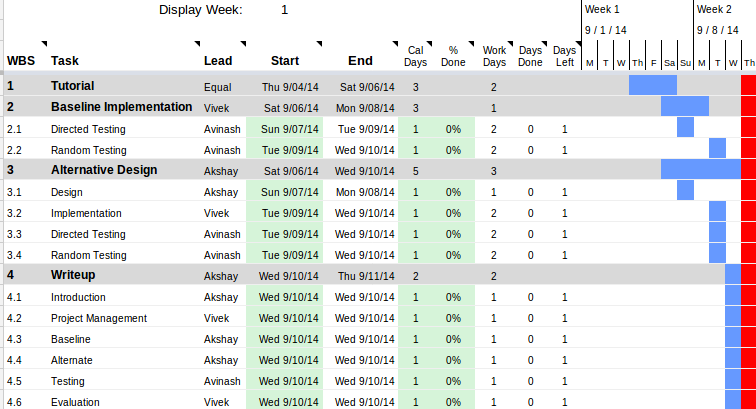
\includegraphics[scale=0.5]{gantt}
\caption{The initial Gantt chart postulating progress}
\label{fig:gantt}
\end{figure}

\begin{figure}
\centering
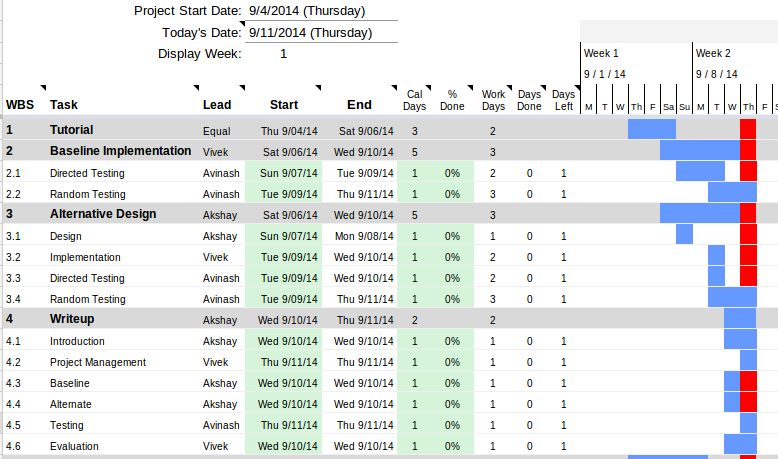
\includegraphics[scale=0.5]{gantt_actual}
\caption{Our actual progress on the lab}
\label{fig:gantt_actual}
\end{figure}



\begin{figure}[b]
\centering
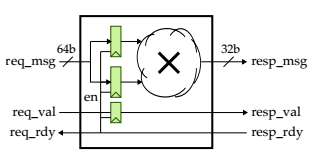
\includegraphics[scale=0.5]{FLmodel}
\caption{Interface for our model. Notice that req/resp,val/rdy signals are part of the val/rdy microprotocol}
\label{fig:model}
\end{figure}

\begin{figure}[b]
\centering
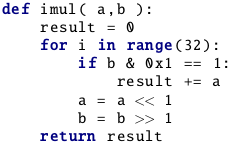
\includegraphics[scale=0.9]{imul}
\caption{Pseudocode for our baseline multiply algorithm}
\label{fig:code}
\end{figure}

\begin{figure}[b]
\centering
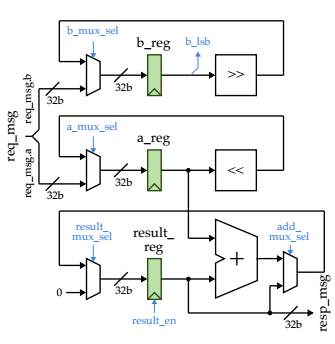
\includegraphics[scale=0.6]{Datapath}
\caption{Datapath Diagram. Again, the structure mimics the pseudocode.}
\label{fig:datapath}
\end{figure}


\end{document}
